%Szablon przygotowany przez mgr Marcina Hanca, z drobnymi zmianami dr Michała Rena
%Master's thesis - Decompiling Android OS applications by Dawid Drozd
\documentclass[12pt,a4paper,leqno,oneside,titlepage]{book}

%%%%%%%%%%%%%%%%%%%%%%%%%%%%%%%%%%%%%%%%%%%%%%%%%%%%%%%%%%%%%%%
%%%%%%%%%%%%%%%%%%%%%%%%%%%%%%%%%%%%%%%%%%%%%%%%%%%%%%%%%%%%%%%
%                      config
%%%%%%%%%%%%%%%%%%%%%%%%%%%%%%%%%%%%%%%%%%%%%%%%%%%%%%%%%%%%%%%
%%%%%%%%%%%%%%%%%%%%%%%%%%%%%%%%%%%%%%%%%%%%%%%%%%%%%%%%%%%%%%%


% Wczytanie pakietów: kodowania, czcionki i języki.
\usepackage[utf8]{inputenc}
\usepackage{lmodern}
\usepackage[english,polish]{babel}
% Wczytanie pakietu 'polski' w celu zapewnienia polskich nazw.
\usepackage{polski}
% Czcionki matematyczne.
\usepackage{amsfonts}
\usepackage{amsmath}

% Ładne początki rozdziałów (pakiet fncychap).
% Polecam Sonny i Conny. Bjornstrup najładniejszy, ale mi się bugował.
\usepackage[Sonny]{fncychap}
% Ładne i klikalne odnośniki.
\usepackage{url}
% Odnośniki dla adresów z polskimi znakami.
\usepackage[]{hyperref}
% Możliwość tworzenia łączonych pól (wg. rzędów) w tabelach.
\usepackage{multirow}
% Pakiet do cytowania kodów źródłowych.
\usepackage{listings}
% Pakiet do ładnego wstawiania grafik.
\usepackage{graphicx}
% Pakiet dodający możliwość wstawienia rozdziału "Akronimy".
\usepackage{acronym}
% Pakiet dodający kolory
\usepackage[usenames,dvipsnames,svgnames,table]{xcolor}
% Pakiet rozwiązujący problem z underscore w Section.
\usepackage[T1]{fontenc}
% Pakiet dodający definicje i twierdzenia.
\usepackage{amsthm}

% Custom format of ARM Assembler source code
\usepackage{package/arm-assembler-latex-listings/lstlangarm}

\frenchspacing

\newcommand{\myAuthorName}{Dawid Patryk Drozd}
\author{\myAuthorName{}}
\title{Dekompilacja aplikacji działających w systemie Android OS.}

% \imod{k} Ładny zapis dzielenia modulo.
\makeatletter
\def\imod#1{\allowbreak\mkern10mu({\operator@font mod}\,\,#1)}
\makeatother

% \rom{n} Liczba n zapisana rzymsko.
\makeatletter
\newcommand*{\rom}[1]{\expandafter\@slowromancap\romannumeral #1@}
\makeatother

% Własne definicje.
% \begin{mydef}
%     Treść definicji.
% \end{mydef}
\newtheorem{mydef}{Definicja}

% Ładny sposób wstawiania cytatu rozpoczynającego rozdział.
% \begin{chapquote}{KTO}
%     CO ONA POWIEDZIAŁA?
% \end{chapquote}
\makeatletter
\renewcommand{\@chapapp}{}
\newenvironment{chapquote}[2][2em]
  {\setlength{\@tempdima}{#1}%
   \def\chapquote@author{#2}%
   \parshape 1 \@tempdima \dimexpr\textwidth-2\@tempdima\relax%
   \itshape}
  {\par\normalfont\hfill--\ \chapquote@author\hspace*{\@tempdima}\par\bigskip}
\makeatother

% Zmiana tekstów w listingach kodów źródłowych na j. polski.
\renewcommand\lstlistingname{Kod źródłowy}
\renewcommand\lstlistlistingname{Spis kodów źródłowych}

% Redefinicja Abstract'ów.
% W celu możliwości wstawienia dwóch na jedną stronę.
\newenvironment{abstractpage}
  {\cleardoublepage\vspace*{\fill}\thispagestyle{empty}}
  {\vfill\cleardoublepage}
\newenvironment{abstract}[1]
  {\bigskip\selectlanguage{#1}%
   \begin{center}\bfseries\abstractname\end{center}}
  {\par\bigskip}

% Dodatkowe definicje stylu stron.
\lstset{
  basicstyle={\small\ttfamily},
  breaklines=true,
  columns=flexible
}

% ToDo marker command
\newcommand{\todo}[1]{\colorbox{yellow}{#1}}

\setlength{\oddsidemargin}{0.5in}
\setlength{\textwidth}{5.7in}
\setlength{\topmargin}{0in}
\setlength{\textheight}{8.5in}
\linespread{1.05}

%%%%%%%%%%%%%%%%%%%%%%%%%%%%%%%%%%%%%%%%%%%%%%%%%%%%%%%%%%%%%%%
%%%%%%%%%%%%%%%%%%%%%%%%%%%%%%%%%%%%%%%%%%%%%%%%%%%%%%%%%%%%%%%
%                      begin{document}
%%%%%%%%%%%%%%%%%%%%%%%%%%%%%%%%%%%%%%%%%%%%%%%%%%%%%%%%%%%%%%%
%%%%%%%%%%%%%%%%%%%%%%%%%%%%%%%%%%%%%%%%%%%%%%%%%%%%%%%%%%%%%%%

% Tu rozpoczyna się zawartość pracy!
\begin{document}

% Strona tytułowa zgodna z wymaganiami:
% http://www.wmi.amu.edu.pl/pl/prace-dyplomowe
\begin{titlepage}
\let\footnotesize\small
\let\footnoterule\relax
\let \footnote \thanks

\begin{center}
{\large \bf Uniwersytet im. Adama Mickiewicza w Poznaniu \\ Wydział Matematyki i~Informatyki \par}
\vspace{0.5cm plus 1mm minus 2mm}
{{\bf Kierunek: Informatyka} \\ \small Specjalizacja:\todo{MISSING!}\par}
\end{center}%

\vspace{1.5cm plus 1fill}
\begin{flushleft}
{\center {\bf \Large \myAuthorName{}} \\ \normalsize Nr albumu: \bf 362617\par}
\end{flushleft}
\vspace{1.5cm plus 1mm minus 2mm}

\begin{center}
{\huge\textbf{Dekompilacja aplikacji działających w systemie Android~OS}\par}
\vspace{0.5cm plus 1mm minus 2mm}
{\large Decompiling Android OS applications}
\par
\vspace{1.5cm plus 1.5fill}

\begin{flushright}\large
\begin{tabular}{l}
Praca magisterska\\[3pt]
\MakeUppercase{ }\\[3pt]
Promotor: \\[3pt]
\bfseries dr Michał Ren \\[3pt]
\end{tabular}
\end{flushright}
\vspace{4cm plus .1fill}
{\large 2017\par}
\end{center}
\end{titlepage}

% Zgłoszenie braku numerowania kolejnych stron.
\pagenumbering{gobble}

\begin{flushright}{
Poznań, dnia 25 czerwca 2017
}\end{flushright}
\begin{center}{
\par
\vspace{1.5cm plus 1.5fill}
{\large OŚWIADCZENIE}
}\end{center}
\par
\vspace{1.5cm plus 1.5fill}
Ja, niżej podpisany \myAuthorName{} student Wydziału Matematyki i~Informatyki Uniwersytetu im. Adama Mickiewicza w Poznaniu oświadczam, że przedkładaną pracę dyplomową pt: ``Dekompilacja aplikacji działających w systemie Android OS'' napisałem samodzielnie. Oznacza to, że przy pisaniu pracy, poza niezbędnymi konsultacjami, nie korzystałem z pomocy innych osób, a~w~szczególności nie zlecałem opracowania rozprawy lub jej części innym osobom, ani nie odpisywałem tej rozprawy lub jej części od innych osób.\\

Oświadczam również, że egzemplarz pracy dyplomowej w~wersji drukowanej jest całkowicie zgodny z~egzemplarzem pracy dyplomowej w~wersji elektronicznej.\\

Jednocześnie przyjmuję do wiadomości, że przypisanie sobie, w~pracy dyplomowej, autorstwa istotnego fragmentu lub innych elementów cudzego utworu lub ustalenia naukowego stanowi podstawę  stwierdzenia  nieważności postępowania w~sprawie nadania tytułu zawodowego.\\

Wyrażam zgodę na udostępnianie mojej pracy w czytelni Archiwum UAM.\\

Wyrażam zgodę na udostępnianie mojej pracy w zakresie koniecznym do ochrony mojego prawa do autorstwa lub praw osób trzecich.
\par
\vspace{1.5cm plus 1.5fill}
\begin{center}{
..............................................\\
{\footnotesize(czytelny podpis studenta)}
}\end{center}


%%%%%%%%%%%%%%%%%%%%%%%%%%%%%%%%%%%%%%%%%%%%%%%%%%%%%%%%%%%%%%%
%%%%%%%%%%%%%%%%%%%%%%%%%%%%%%%%%%%%%%%%%%%%%%%%%%%%%%%%%%%%%%%
%                      Thanks to...
%%%%%%%%%%%%%%%%%%%%%%%%%%%%%%%%%%%%%%%%%%%%%%%%%%%%%%%%%%%%%%%
%%%%%%%%%%%%%%%%%%%%%%%%%%%%%%%%%%%%%%%%%%%%%%%%%%%%%%%%%%%%%%%

\newpage

\phantom{.}

\vspace{12cm} \hspace{1cm}\phantom{.}\\
\phantom{.}\hspace{5cm}{Składam serdeczne podziękowania}\\
\phantom{.}\hspace{5cm}{doktorowi }\\
\phantom{.}\hspace{5cm}{Michałowi Renowi }\\
\phantom{.}\hspace{5cm}{za jego nieocenioną pomoc }\\
\phantom{.}\hspace{5cm}{przy pisaniu tej pracy.}\\
\phantom{.}\hspace{5cm}{}\\
\phantom{.}\hspace{5cm}{Dziękuję również}\\
\phantom{.}\hspace{5cm}{Marcinowi Hancowi za szablon i }\\
\phantom{.}\hspace{5cm}{za owocną, naukową współpracę}\\
\phantom{.}\hspace{5cm}{przy tworzeniu wyników z tej pracy.}\\


%%%%%%%%%%%%%%%%%%%%%%%%%%%%%%%%%%%%%%%%%%%%%%%%%%%%%%%%%%%%%%%
%%%%%%%%%%%%%%%%%%%%%%%%%%%%%%%%%%%%%%%%%%%%%%%%%%%%%%%%%%%%%%%
%                      Bookmarks
%%%%%%%%%%%%%%%%%%%%%%%%%%%%%%%%%%%%%%%%%%%%%%%%%%%%%%%%%%%%%%%
%%%%%%%%%%%%%%%%%%%%%%%%%%%%%%%%%%%%%%%%%%%%%%%%%%%%%%%%%%%%%%%

\newpage
% Przód pracy - spisy i abstrakty.
\frontmatter
% Spis treści ze specjalnym uwzględnieniem podkreśleń w tytułach sekcji.
\pagestyle{plain}
{
    \catcode`\_=12
    \tableofcontents
}
% Spis ilustracji.
\listoffigures
% Spis tabeli.
\listoftables
% Spis listingów kodów źródłowych.
\begingroup
\let\clearpage\relax
\lstlistoflistings
\endgroup

%%%%%%%%%%%%%%%%%%%%%%%%%%%%%%%%%%%%%%%%%%%%%%%%%%%%%%%%%%%%%%%
%%%%%%%%%%%%%%%%%%%%%%%%%%%%%%%%%%%%%%%%%%%%%%%%%%%%%%%%%%%%%%%
%                      Abstract
%%%%%%%%%%%%%%%%%%%%%%%%%%%%%%%%%%%%%%%%%%%%%%%%%%%%%%%%%%%%%%%
%%%%%%%%%%%%%%%%%%%%%%%%%%%%%%%%%%%%%%%%%%%%%%%%%%%%%%%%%%%%%%%

% Strona z abstraktami.
\begin{abstractpage}
% Abstrakt w języku polskim.
\begin{abstract}{polish}
Celem pracy jest omówienie procesu dekompilacji aplikacji mobilnych pisanych na system operacyjny Android.
Na początku poznamy budowę aplikacji androidowej. Korzystając z tej wiedzy nauczymy się obsługi narzędzi które ułatwiają proces dekompilacji. Dzięki narzędzią otrzymamy wynik desasemblacji i nauczymy się go interpretować. Z tak otrzymanego wyniku postaramy się poskładać wszystko z powrotem do działającej aplikacji. Dowiemy się jak system Android identyfikuje i weryfikuje pochodzenie aplikacji. Na koniec dowiemy się jakie niebezpieczeństwo niesie za sobą źle zabezpieczony kod aplikacji. Prześledzimy proces który utrudnia odzyskiwanie kodu źródłowego za pomocę technik odwrotnej inżynierii.
 
\end{abstract}
\smallskip
\noindent \textbf{Słowa~kluczowe:} RE, reverse engineering, inżynieria odwrotna, dekompilacja, android, apk, apktool, smali, obfuskacja, zaciemnianie kodu, dezasemblacja, deasembler, disassembler, objdump, asembler, dekompilator

%Abstrakt w języku angielskim.
\begin{abstract}{english}
\todo{translate when PL is done}
\end{abstract}
\smallskip
\noindent \textbf{Keywords:} \todo{translate when PL is done}
\end{abstractpage}

% Finally - PRACA!
\mainmatter

%%%%%%%%%%%%%%%%%%%%%%%%%%%%%%%%%%%%%%%%%%%%%%%%%%%%%%%%%%%%%%%
%%%%%%%%%%%%%%%%%%%%%%%%%%%%%%%%%%%%%%%%%%%%%%%%%%%%%%%%%%%%%%%
%                      Introduction
%%%%%%%%%%%%%%%%%%%%%%%%%%%%%%%%%%%%%%%%%%%%%%%%%%%%%%%%%%%%%%%
%%%%%%%%%%%%%%%%%%%%%%%%%%%%%%%%%%%%%%%%%%%%%%%%%%%%%%%%%%%%%%%

% Wstęp jest uwzględniony w spisie treści jako rozdział bez numeru.
\addcontentsline{toc}{chapter}{Wstęp}
\chapter*{Wstęp}

Inżynieria wsteczna (ang. \emph{reverse engineering}, w skrócie RE) jest procesem analizy budowy i sposobu działania oprogramowania. Proces ten jest często długim procesem ze względu na to, że analizujemy kod który poprzednio został przekształcony przez inne programy (kompilatory, preprocesory, itp.) do formy mniej czytelnej. Takim przykładem może być skompilowany program napisany w C++.


\lstinputlisting[language=C++, captionpos=b, belowcaptionskip=4pt, caption={Przykładowy program w C++}]{src/sample.cpp}

Uproszczony kod po odwrotnej inzynierii dla platformy ARM. 

\lstinputlisting[language={[ARM]Assembler}, captionpos=b, belowcaptionskip=4pt, caption={Zdesasemblowany przykładowy kod}]{src/sample.s}

Przykład choć krótki to już pokazuje jak mamy utrudnione zadanie. Często analizujemy kod który jest bardziej zrozumiały dla maszyny niż człowieka.

Proces inżynieri wstecznej jest dodatkowo utrudniany przez programistów którzy nie chcą by ktoś podglądał jak pewna funkcjonalność zastała zrealizowana. W tym celu stosowana jest obfuskacja kodu. Jednak inżynieria wsteczna czasem jest jedynym sposobem na dowiedzenie się jak coś działa. Przykładem może być brak kodu źródłowgo pewnej biblioteki jak i brak dokumentacji do niej. Innym przykładem może być chęć dodania lub naprawienia pewnej funkcjonalności. Producent mógł porzucić rozwój oprogramowania a nasza organizacja z pewnych powodów nie może zmienić tej biblioteki.

Celem tej pracy jest przedstawienie narzędzi jak i procesu dekompilacji zbudowanych aplikacji i ponownej kompilacji zmodyfikowanej aplikacji na system operacyjny Android.


%%%%%%%%%%%%%%%%%%%%%%%%%%%%%%%%%%%%%%%%%%%%%%%%%%%%%%%%%%%%%%%
%%%%%%%%%%%%%%%%%%%%%%%%%%%%%%%%%%%%%%%%%%%%%%%%%%%%%%%%%%%%%%%
%                      chapter
%%%%%%%%%%%%%%%%%%%%%%%%%%%%%%%%%%%%%%%%%%%%%%%%%%%%%%%%%%%%%%%
%%%%%%%%%%%%%%%%%%%%%%%%%%%%%%%%%%%%%%%%%%%%%%%%%%%%%%%%%%%%%%%

\chapter{Jak zbudowana jest aplikacja na Android'a}
\section{Format .apk}

Rozszerzenie nazwy pliku bierze sie z \emph{Android Package Kit (APK)}.
Format pliku przypomina ten znany z plików .jar
Pliki oznaczone tym rozszerzeniem slużą do rozpowszechniania aplikacji na system android. Na skład paczki .apk wchodzą:

\begin{itemize}
\item skompilowany kod Java w formacie .dex
\item zasoby takie jak png czy mp3
\item certyfikaty
\item plik manifestu
\end{itemize}

Nazwa pliku jest dowolna pod warunkiem, że jest zakończona przez .apk
Pliki APK są pewnego roadzaju archiwum które bazuje na formacie ZIP.

\begin{figure}[h!]
	\centering
	\includegraphics[height=0.3\textheight]{img/apk_content_as_zip.png}
	\caption{Otworzony plik .apk za pomocą programu ark}
\end{figure}

Szczegółowa budowa paczki apk:
\begin{itemize}
\item \texttt{Katalog META\_INF}

\begin{figure}[h!]
	\centering
	\includegraphics[height=0.3\textheight]{img/apk_content_as_zip_meta_inf.png}
	\caption{META INF w ark}
\end{figure}

W katalogu znajduje się plik MANIFEST.MF. Plik ten zawiera metadane dotyczące zawartości paczki:

Przykład:

\begin{lstlisting}
Manifest-Version: 1.0
Built-By: Generated-by-ADT
Created-By: Android Gradle 2.3.3

Name: res/drawable-hdpi-v4/abc_list_longpressed_holo.9.png
SHA1-Digest: KQunCQh0E4bP0utgN0cHdQr9OwA=

Name: res/drawable-xxhdpi-v4/abc_ic_star_half_black_16dp.png
SHA1-Digest: EikVyBT5I7pmbJO2k8qF0V5hUc0=

Name: res/drawable-hdpi-v4/com_facebook_tooltip_black_background.9.png
SHA1-Digest: +DxTpyUKpT11iz68MG1Q0iB2EvA=

Name: res/drawable/common_google_signin_btn_icon_dark_normal.xml
SHA1-Digest: Qa00to2cn7JphS3q33GWp3lxTUs=
\end{lstlisting}

\item CERT.RSA - certyfikat aplikacji
\item CERT.SF
Lista zasobów i ich SHA-1 skład jest taki sam jak w przypadku MANIFEST.MF


\item Folder lib
Katalog opcjonalny w którym powinny znajdować się skompilowane biblioteki natywne na daną platformę np. armeabi, x86, mips

\item AndroidManifest.xml - dodatkowy plik manifestu który zawiera między innymi nazwy, wersję i prawa aplikacji. Plik ten często jest binarnym XML który łatwo zamienić na formę czytelną dla człowieka.

\item resources.arsc - plik zawierający prekompilowane zasoby takie jak binarne XML

\item folder assets
Folder który zawiera zasoby które nie są poddane dodatkowym obróbką przez proces budowania apk.

\item folder res
Folder zawiera zasoby które nie zostały przetworzone i dołączone do pliku resources.arsc

\item classes.dex Skompilowane pliki Java do formatu .dex które rozumie Dalvik virtual machine

\end{itemize}

%%%%%%%%%%%%%%%%%%%%%%%%%%%%%%%%%%%%%%%%%%%%%%%%%%%%%%%%%%%%%%%
%%%%%%%%%%%%%%%%%%%%%%%%%%%%%%%%%%%%%%%%%%%%%%%%%%%%%%%%%%%%%%%
%                      chapter
%%%%%%%%%%%%%%%%%%%%%%%%%%%%%%%%%%%%%%%%%%%%%%%%%%%%%%%%%%%%%%%
%%%%%%%%%%%%%%%%%%%%%%%%%%%%%%%%%%%%%%%%%%%%%%%%%%%%%%%%%%%%%%%

\chapter{Narzędzia do dekompilacji}

\section{apktool}

Narzędzie to służy do przeprowadzenia odwrotnej inżynierii na wskazanym pliku apk. Potrafi zdekodować źródła aplikacji do formy zbliżonej przed jej zbudowaniem. Wiele procesów zostało zautomatyzowanych takich jak zbudowanie ponowne aplikacji z zdekompilowanych źródeł. \\
\lstinline|apktool| jest otwarto źródłowym oprogramowaniem na licencji \mbox{Apache 2.0 License.} \\
\\
Kod narzędzia jest dostępny na: \url{https://github.com/iBotPeaches/Apktool} \newline
Strona narzędzia: \url{https://ibotpeaches.github.io/Apktool/}
\newline
\newline
Aplikacja jest napisana w języku Java dzięki czemu działa bezproblemowo na większości systemach operacyjnych. Jest to aplikacja bez interfejsu graficznego. Działa w konsoli.
\newline
\subsection{Dekompilacja}
Przykład użycia zostanie zaprezentowany na przykładowej aplikacji. Zakładając, że mamy już dostępną naszą \lstinline|.apk|\\
\begin{lstlisting}[language=bash]
{master} ~/Projects/UAM/
$ cd apktool
{master} ~/Projects/UAM/msc/apktool
$ ./apktool d ../sample-android-app/Thesis/app/app-release.apk 
I: Using Apktool 2.2.3 on app-release.apk
I: Loading resource table...
I: Decoding AndroidManifest.xml with resources...
I: Loading resource table from file: /home/gelldur/.local/share/apktool/framework/1.apk
I: Regular manifest package...
I: Decoding file-resources...
I: Decoding values */* XMLs...
I: Baksmaling classes.dex...
I: Copying assets and libs...
I: Copying unknown files...
I: Copying original files...
\end{lstlisting}
Dzięki tej komendzie uzyskamy źródła z naszej aplikacji. 
\begin{figure}[h!]
	\centering
	\includegraphics[height=0.3\textheight]{img/apktool/sample_apk.png}
	\caption{Wynik pracy \lstinline|apktool d app-release.apk|}
\end{figure}
\begin{itemize}
\item{Folder smali}\\
Zawiera odzyskane inżynierią wsteczną kody źródłowe naszej aplikacji. Kody jednak nie będą w języku Java a w Smali. Smali jest omówiony w \ref{smali}.
\item{Folder original}\\
Zawiera oryginalne źródła z naszego \lstinline|.apk| takie jak oryginalny \lstinline|AndroidManifest.xml| czy  \lstinline|META-INF|
\item{Folder lib}\\
Zwiera natywne biblioteki wykorzystywane przez aplikację. W naszym przykładzie jest to skompilowana dynamiczna biblioteka z jedną prostą funkcją. Oby odzyskać kod natywny musielibyśmy sięgnąć do innych narzędzi.
\item{Folder res}\\
Zawiera wszystkie oryginalne zasoby naszej aplikacji które zostały wcześniej przetworzone i w odpowiedni sposób upakowane.
\item{AndroidManifest.xml}\\
Zdekodowany \lstinline|AndroidManifest.xml|. Tak prezentuje się diff manifestu przed i po zdekodowaniu:

\begin{figure}[h!]
	\centering
	\includegraphics[height=0.3\textheight]
	{img/apktool/sample_diff_manifest.png}
	\caption{Diff między AndroidManifest.xml z źródeł a odzyskanym z pliku .apk}
\end{figure}

\item{apktool.yml}\\
Plik z metadanymi od apktool.
\end{itemize}

\subsection{Budowanie z powrotem}
Aplikację możemy zbudować ponownie z naszych zasobów. Przykład tego zastosowania znajduje się poniżej.

\begin{lstlisting}[language=bash]
{master} ~/Projects/UAM/msc/apktool
$ ./apktool b ./app-release/
I: Using Apktool 2.2.3
I: Checking whether sources has changed...
I: Smaling smali folder into classes.dex...
I: Checking whether resources has changed...
I: Building resources...
I: Copying libs... (/lib)
I: Building apk file...
I: Copying unknown files/dir...
\end{lstlisting}
W taki sposób otrzymamy znowu zbudowaną aplikację jednak nie będzie ona podpisana tym samym kluczem. Jaki wpływ na aplikację ma podpisaniem kluczem jest omówione w \ref{signing} rozdziale.

\section{dex2jar}

% https://github.com/pxb1988/dex2jar

\section{apkToJava}

% https://github.com/ajitsing/apkToJava


%%%%%%%%%%%%%%%%%%%%%%%%%%%%%%%%%%%%%%%%%%%%%%%%%%%%%%%%%%%%%%%
%%%%%%%%%%%%%%%%%%%%%%%%%%%%%%%%%%%%%%%%%%%%%%%%%%%%%%%%%%%%%%%
%                      chapter
%%%%%%%%%%%%%%%%%%%%%%%%%%%%%%%%%%%%%%%%%%%%%%%%%%%%%%%%%%%%%%%
%%%%%%%%%%%%%%%%%%%%%%%%%%%%%%%%%%%%%%%%%%%%%%%%%%%%%%%%%%%%%%%
%- Zabezpieczenia przed modyfikowaniem aplikacji (podpisywanie apki certyfikatem,nazwa package apki)

\chapter{Identyfikacja i weryfikowanie aplikacji}
\section{Nazwa paczki}



\section{Cyfrowy podpis}
\label{signing}

%%%%%%%%%%%%%%%%%%%%%%%%%%%%%%%%%%%%%%%%%%%%%%%%%%%%%%%%%%%%%%%
%%%%%%%%%%%%%%%%%%%%%%%%%%%%%%%%%%%%%%%%%%%%%%%%%%%%%%%%%%%%%%%
%                      chapter
%%%%%%%%%%%%%%%%%%%%%%%%%%%%%%%%%%%%%%%%%%%%%%%%%%%%%%%%%%%%%%%
%%%%%%%%%%%%%%%%%%%%%%%%%%%%%%%%%%%%%%%%%%%%%%%%%%%%%%%%%%%%%%%

\chapter{Wynik desasemblacji}

\begin{figure}[h!]
	\centering
	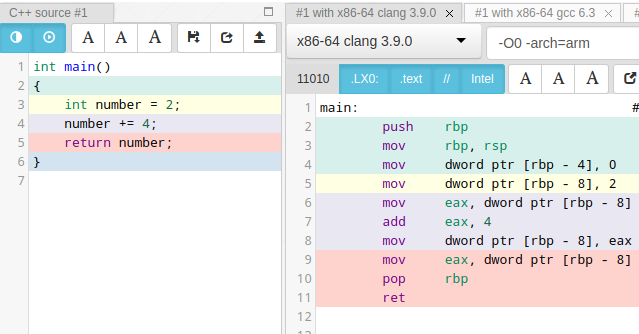
\includegraphics[height=0.3\textheight]{img/Screenshot_godbolt_org-sample.png}
	\caption{Wygenerowany przykład z strony \url{godbolt.org}}
\end{figure}


\section{SMALI}
\label{smali}

\section{Dalvik/ART bytecode}

%%%%%%%%%%%%%%%%%%%%%%%%%%%%%%%%%%%%%%%%%%%%%%%%%%%%%%%%%%%%%%%
%%%%%%%%%%%%%%%%%%%%%%%%%%%%%%%%%%%%%%%%%%%%%%%%%%%%%%%%%%%%%%%
%                      chapter
%%%%%%%%%%%%%%%%%%%%%%%%%%%%%%%%%%%%%%%%%%%%%%%%%%%%%%%%%%%%%%%
%%%%%%%%%%%%%%%%%%%%%%%%%%%%%%%%%%%%%%%%%%%%%%%%%%%%%%%%%%%%%%%

\chapter{Sposoby ochrony przed desasemblacją}
\section{Obfuskacja}
\section{Proguard}
\section{Natywny kod}

%%%%%%%%%%%%%%%%%%%%%%%%%%%%%%%%%%%%%%%%%%%%%%%%%%%%%%%%%%%%%%%
%%%%%%%%%%%%%%%%%%%%%%%%%%%%%%%%%%%%%%%%%%%%%%%%%%%%%%%%%%%%%%%
%                      chapter
%%%%%%%%%%%%%%%%%%%%%%%%%%%%%%%%%%%%%%%%%%%%%%%%%%%%%%%%%%%%%%%
%%%%%%%%%%%%%%%%%%%%%%%%%%%%%%%%%%%%%%%%%%%%%%%%%%%%%%%%%%%%%%%

%- Zabezpieczenia / Niebezpieczeństwa. Np wstrzykiwanie w zapytania do serwera. (Ogólnie omówić czemu warto/trzeba zabezpieczyć kod przed dekompilacją)
\chapter{Niebezpieczeństwa źle zabezpieczonego kodu}

%%%%%%%%%%%%%%%%%%%%%%%%%%%%%%%%%%%%%%%%%%%%%%%%%%%%%%%%%%%%%%%
%%%%%%%%%%%%%%%%%%%%%%%%%%%%%%%%%%%%%%%%%%%%%%%%%%%%%%%%%%%%%%%
%                      chapter
%%%%%%%%%%%%%%%%%%%%%%%%%%%%%%%%%%%%%%%%%%%%%%%%%%%%%%%%%%%%%%%
%%%%%%%%%%%%%%%%%%%%%%%%%%%%%%%%%%%%%%%%%%%%%%%%%%%%%%%%%%%%%%%

\chapter{Projekt}

%%%%%%%%%%%%%%%%%%%%%%%%%%%%%%%%%%%%%%%%%%%%%%%%%%%%%%%%%%%%%%%
%%%%%%%%%%%%%%%%%%%%%%%%%%%%%%%%%%%%%%%%%%%%%%%%%%%%%%%%%%%%%%%
%                      chapter
%%%%%%%%%%%%%%%%%%%%%%%%%%%%%%%%%%%%%%%%%%%%%%%%%%%%%%%%%%%%%%%
%%%%%%%%%%%%%%%%%%%%%%%%%%%%%%%%%%%%%%%%%%%%%%%%%%%%%%%%%%%%%%%

%\chapter{Bibliografia}
\newpage
% Dodanie wpisu Bibliografia do Spisu Treści.
\addcontentsline{toc}{chapter}{Bibliografia}
% Styl bibliografii: unsrt lub plain
\bibliographystyle{plain}
\bibliography{bibliografia}

%%%%%%%%%%%%%%%%%%%%%%%%%%%%%%%%%%%%%%%%%%%%%%%%%%%%%%%%%%%%%%%
%%%%%%%%%%%%%%%%%%%%%%%%%%%%%%%%%%%%%%%%%%%%%%%%%%%%%%%%%%%%%%%
%%%%%%%%%%%%%%%%%%%%%%%%%%%%%%%%%%%%%%%%%%%%%%%%%%%%%%%%%%%%%%%
%%%%%%%%%%%%%%%%%%%%%%%%%%%%%%%%%%%%%%%%%%%%%%%%%%%%%%%%%%%%%%%
%%%%%%%%%%%%%%%%%%%%%%%%%%%%%%%%%%%%%%%%%%%%%%%%%%%%%%%%%%%%%%%
%%%%%%%%%%%%%%%%%%%%%%%%%%%%%%%%%%%%%%%%%%%%%%%%%%%%%%%%%%%%%%%
%%%%%%%%%%%%%%%%%%%%%%%%%%%%%%%%%%%%%%%%%%%%%%%%%%%%%%%%%%%%%%%
%%%%%%%%%%%%%%%%%%%%%%%%%%%%%%%%%%%%%%%%%%%%%%%%%%%%%%%%%%%%%%%

% Spis akronimów użytych w pracy
\chapter*{Akronimy}
\begin{acronym}
\acro{KISS}{Keep It Simple Stupid}
\acro{RE}{reverse engineering}
\acro{IT}{Information Technology}
\acro{APK}{Android Package}
\end{acronym}
\end{document}
